\documentclass[12pt]{book}
\usepackage{diffyqssetupUB}

\begin{document}

%{\color{red}Suspected erroneous material.}
%{\color{teal}JR: Comment preceded by author's initials.}
%{\color{blue}Suggested revised version.}

%extra exercises {Integrals as solutions}
\begin{exercise}
%http://math.buffalo.edu/306/2019_06_13/001
Find the general solution of $y' = \frac{1}{x^2-2x-8}$
\end{exercise}
{\color{teal}BH ok; soln $y \left( x \right) =-1/6\,\ln  \left( x+2 \right) +1/6\,\ln  \left( x-
4 \right) +{\it \_C1}$
}
{\color{teal}BH removed repeat of exercise}

\begin{exercise}
%http://math.buffalo.edu/306/2019_06_13/002
Find the general solution of $y' = \frac{1}{x^4 + 4x^2}$
\end{exercise}
{\color{teal}BH ok; 
$y \left( x \right) =-1/4\,{x}^{-1}-1/8\,\arctan \left( 1/2\,x \right) 
+{\it \_C1}$}

%\setcounter{exercise}{150}
\begin{exercise}
%http://math.buffalo.edu/306/2019_06_13/003
Find the general solution to the following differential equations (DEs) by integration:
\begin{enumerate}[a)]
    \item $\frac{d^2y}{dx^2} = 4x^3+ e^{2x}$
    \item $\frac{d^3y}{dx^3} = 6x^2 +1$
    \item $\frac{d^3y}{dx^3}= \cos(2x)$
\end{enumerate}
\end{exercise}

\exsol{%
\begin{enumerate}[a)]
    \item $y = \frac{x^5}{5} +\frac{e^{2x}}{4} + Cx + D$
    \item {\color{blue}$y = \frac{x^5}{10} +\frac{x^3}{6} + Cx^2 + Dx +E$}
    \item $y = -\frac{\sin(2x)}{8} + Cx^2 + Dx +E$
\end{enumerate}
{\color{teal}BH ok}
}

\begin{exercise}
%http://math.buffalo.edu/306/2019_06_13/004
Find the particular solution to the following initial value problems (IVPs):
\begin{enumerate}[a)]
    \item $y'' = 6x + 2 ;\ y(1) = -1,\ y'(1)=7$
    \item $y'' = e^{\frac{1}{3}x} ;\ y(0) = -2,\ y'(0)=4$
    \item $y'' =\frac{1}{\sqrt{x+9}} ;\ y(0) = 10,\ y'(0)=1$
\end{enumerate}
\end{exercise}

\exsol{%
\begin{enumerate}[a)]
    \item $y = x^3+x^2+2x-5$
    \item {\color{blue}$y = 9e^{\frac{1}{3}x}+x-11$}
    \item {\color{blue}$y = \frac{4}{3}(x+9)^{3/2}-5x-26$}
\end{enumerate}
{\color{teal}BH all ok}
}

%extra exercises {Slope fields}
%\setcounter{exercise}{50}
\begin{exercise}
%http://math.buffalo.edu/306/2019_06_13/005
{\color{blue}
Sketch the region of continuity for $f(x,y)$ on a set of axes and sketch the region of continuity for $\frac{\partial f}{\partial y}(x,y)$ on a separate set of axes.
}
{\color{teal}BH expanded the statement to clarify; JJ ok}
Apply Picard's Theorem to determine whether the solution exists and whether it is unique.

\begin{enumerate}[a)]
    \item $y' = 2x^2y + 3xy^2\ , \, y(1)=2$
    \item $y' = \frac{1}{x+y}\ , \, y(-1) = 3$
    {\color{teal}BH $\frac{1}{x+y}$ would work just as well}
    \item $y' = \sqrt{2x-3y} \ , \, y(3)=2$
    \item $y' = \sqrt[3]{2y+6x} \ , \, y(1)=-3$
    \item $y' = x \ln(y) \ , \,  y(2)=3$
    \item $y' = x^2 e^y \ , \, y(-1)=4$
    \item $y' = \sqrt{5y+10x} \ ,\,  y(1)=0$
    \item $y' = \sqrt{5y+10x} \ , \, y(1)=-2$
    \item $y' = 2y^{\frac{1}{3}} \ , \, y(0)=0$
    \item $y' = 2y^{\frac{1}{3}} \ , \, y(-1)=-2$
\end{enumerate}

\end{exercise}

\begin{exercise}
%http://math.buffalo.edu/306/2019_06_13/006
{\color{red}
Sketch the region of continuity for $f(x,y)$ and $\frac{\partial f}{\partial y}(x,y)$.
}
{\color{blue}
Sketch, on one single set of axes, the region where both $f(x,y)$ and $\frac{\partial f}{\partial y}(x,y)$
are continuous.
}
Determine the conditions on $(x_0,y_0)$ for which Picard's Theorem guarantees that a unique solution exists. 
{\color{teal}BH, JJ ok}

\begin{enumerate}[a)]
    \item $y' = \sqrt{2x-y}$
    \item $y' = \ln(y-x^2)$
    \item $y' = \sqrt{y} \ln(x)$
    \item $y' = \sqrt[3]{x^2-y}$
    \item $y' = \frac{3x+2y}{x^2 - y^2}$
\end{enumerate}


\end{exercise}
\vspace{5mm}
%extra material {Separable equations}
% After Example 1.3.4

\begin{example}\label{Separaeq:expogrowth} \textbf{Exponential growth $x'=kx,\ k>0$}
\vspace{5mm}

A culture initially contains 20,000 bacteria. After 5 hours there are 400,000 bacteria. Determine the function $P(t)$ expressing population as a function of time $t$ (in hours).
What is the rate of growth when the population is 1 million bacteria?
{\color{blue}
Round to the nearest $1000$ bacteria/hour.
}

\vspace{3mm}

The population is given by the separable DE:
$$P'=kP$$
with the IC: $$P(0)=20,\!000.$$\\
Solving,
\begin{align*}
    \frac{dP}{P} & = k dt\\
    \ln P &= kt + C
    \\
    P(t) &= P_0 e^{kt}\ \text{ where } 
    {\color{blue} P_0 = P(0) = 20,\!000. }
\end{align*}

To find the growth constant $k$:
    {\color{blue}
\begin{align*}
    P(5) &= 400,\!000 = 20,\!000 e^{k (5)}\\
    k &= \frac{\ln 20}{5} \, (\text{hr})^{-1}
\end{align*}
}
{\color{teal}BH 
rate constant to 2 digits? It happens $ln(20)/5 appx. 0.5991464548$
JJ sig figs? trailing zeros give order of magnitude accuracy
BH yes- the trailing zero in 0.60 is intended to mean between 0.595 and 0.605.
Another possible choice would be 0.599, meaning between 0.5985 and 0.5995 and 0.5991, but 0.599 is ugly.
}
{\color{teal}BH The answer 600,000 bacteria/hour conceals the accuracy of the
result, and the $10^4$ matches the $10^6$
BH Specify round to the nearest 1000 bacteria/hour
so answer can be 599,000 rather that 600,000}
Then 
{\color{blue}
$P(t) = 20,\!000 e^{kt}$
}
\vspace{3mm}

At the time $t$ when $P(t) = 10^6$ bacteria, the growth rate of the population is:
$$P'= k P = \frac{\ln{20}}{5}(10^6) \approx 
{\color{red}
\text{600,000}}
{\color{blue} 599,\!000}\  \text{bacteria/hour}$$

\end{example}

\begin{example}\label{Separaeq:expodecay}
\textbf{Exponential decay $x' = -\lambda x,\ \lambda>0.$}
\vspace{5mm}

A sandal made of a cedar was found in an archaeological excavation at Uruk in Mesopotamia. A radiochemical analysis showed that the sandal contained 54\% of the radioactive isotope ${}^{14}\text{C}$  present in a living cedar tree. How old is the sandal? Round to the nearest century.
\newline

{\color{blue}
Let $S(t) = $ amount of ${}^{14}\text{C}$ present at $t$ years after the sandal
was made, 
and suppose $\lambda=0.00012 \, (\text{yr})^{-1}$ is the decay constant for 
${}^{14}\text{C}$. Then
\begin{align*}
S(t) &= S_0 e^{-0.00012 t}\\
S(t) &= 0.54 S_0 = S_0 e^{-0.00012t},\\
t &= \frac{\ln 0.54}{-0.00012} \approx \text{5100}\ \text{years.}
\end{align*}
}
{\color{teal}BH Wiki half-life of Carbon 14 is $5,730 \pm 40$ years:
Possible values for $\lambda$
$\lambda_1 = ln(2)/5690 = 0.0001218184851$,
$\lambda_2 = ln(2)/5730 = 0.0001209680943$,
$\lambda_3 = ln(2)/5770 = 0.0001201294940$ 
In all cases 0.00012 is a correctly rounded approximation
but the $5135$ could be $\pm 35$, (say)
JJ Edwards and Penney use 0.0001216. Use $\lambda_1?$
BH Using 0.0001216 is claiming 0.00012155 to 0.00012165,
off-center and an interval of width 0.00000005 which is much smaller than the actual interval width 0.0000017.
Using $\lambda_1 = 0.0001218$ would be similarly
off-center and claiming too much accuracy.
Using 0.000121 would be not too bad, since
0.0001205 to 0.0001215 is pretty well centered
on $[\lambda_1,\lambda_3]$
and the interval width 0.0000005 is smaller than
the actual interval only by a factor of 3
}
\end{example}

\vspace{5mm}
%extra exercises {Separable equations}
%\setcounter{section}{3}
%\setcounter{exercise}{50}
\begin{exercise}
%http://math.buffalo.edu/306/2019_06_21/001
{\color{blue}
Sixteen grams of a radioactive substance decays to twelve grams in 500 years.
Let $S(t)$ be the number of grams remaining at time $t$ years.
}
\begin{enumerate}[a)]
    \item Find the decay constant of this substance. Determine the exact value and an approximation.
    \item What is the half-life of the radioactive substance?
    \item How much will remain after 1000 years? What is the \textbf{rate of disintegration} at this time?
\end{enumerate}
\end{exercise}
{\color{teal}BH changed P(t) to $S(t)$ and 300 years to 500 years. 
Issue: with 300 years, the half-life is 723 years, and no known isotope
has this half-life. With instead 500 years, the half-life becomes 1205 years, 
and holmium-166 (metastable) has half-life 1200 years. 
Also, 500 instead of 300 opens up an alternate method of figuring out the amount that remains after 1000 years, since 1000=2(500)
JJ check Values chosen were not intended to correspond to
an actual isotope. This is better
}

\begin{exercise}
%http://math.buffalo.edu/306/2019_06_21/002
Let P(t) be the population of a certain species of insect at time $t,$ where $t$ is measured in days.
Suppose a population of 30,000 insects grows to 150,000 in 3 days.
\begin{enumerate}[a)]
    \item Find the growth constant for this population.
    \item Write the corresponding initial value problem (DE and IC) and its solution.
    \item How long will it take for the population to triple?
\end{enumerate}
\end{exercise}

\begin{exercise}
%http://math.buffalo.edu/306/2019_06_21/003
Suppose that \$10,000 is invested at 5.5\% interest. Let $A(t)$ be the amount in this account at time $t$ years.
\begin{enumerate}[a)]
    \item Write the DE, IC and solution for this problem.
    \item How much is in the account after 5 years? What is the rate of growth at this time?
    \item When there is \$20,000 in the account, what is the rate of growth?
    \item When will the original amount triple?
\end{enumerate}
\end{exercise}

\begin{exercise}
%http://math.buffalo.edu/306/2019_06_21/004
Assume that the motion of a car is subject to a combined resistive force due to friction and wind resistance.
Newton's Second Law gives $m\,v' = r\,v$ or $v'=-k\,v$.
\begin{enumerate}[a)]
    \item The car is moving with a constant speed on a straight road at 70 mph when the engine suddenly stops.
    {\color{blue}
    At 1 minute after the engine has stopped, the speed of the car is 56 mph. Solve the IVP for $v(t)$.
    }
    \item Determine the position function $x(t)$.
    \item 
    {\color{blue}After the engine stops, how far does the car go before it stops moving?
    }
\end{enumerate}
{\color{teal}BH changed speed at engine stop from 53 mph to 56 mph so numbers work out more simply
JJ check}
{\color{teal}BH engine stall changed to engine stops, slight rephrasing}
\end{exercise}

\begin{exercise}
%http://math.buffalo.edu/306/2019_06_21/005
In 1982, a local sponge diver discovered a shipwreck off the coast of Uluburun in south-western Turkey.
Dendrochronology dated the ship in the late Bronze Age, about 1305 B.C.E. If a radiochemical assay had been 
performed in 2010 on a wooden writing tablet recovered from the shipwreck, what percentage of ${}^{14}\text{C}$
would have been found in the tablet? 
{\color{blue}
Round to the nearest percent. Use the value $\lambda = 0.00012 \, (\text{yr})^{-1}$ for the decay constant of ${}^{14}\text{C}$.
}
{\color{teal}BH see previous cedar sandal for
discussion of carbon 14 half-life and
decay constant JJ check Use $\lambda_1?$
}

\end{exercise}

\exsol{%
{\color{blue}
$100 e^{- 0.00012 \times 3315} \approx 67\%$
}
}

\begin{exercise}
%http://math.buffalo.edu/306/2019_06_21/006
A long-term investment account guarantees 3\% annual interest. %  [Modified by JR 1/5/20]per year. on the initial amount invested.
\begin{enumerate}[a)]
    \item How long would it take for the initial amount to double?
    \item What should be invested initially, if one wishes to have \$250,000 in 25 years?
\end{enumerate}
\end{exercise}

\exsol{%
{\color{blue}
\begin{enumerate}[a)]
    \item $\frac{100}{3}\ln{2} \approx 23.1$ yr
    \item $250000 e^{-3/4}\approx \$118,092$
\end{enumerate}
}
}

\begin{exercise}
%http://math.buffalo.edu/306/2019_06_21/007
A radioactive substance decays to $4/5$ of its original mass in 
{\color{blue}7} years. What is the half-life of this 
substance?
{\color{teal}BH: changed original value of 23 years to 7 years, 
so that the half-life in this example
works out to be very close to that of an actual radioactive 
substance, Actinium}

\end{exercise}

\exsol{%
{\color{blue}
$7 \ln(2)/\ln(5/4) \approx 21.7$ yr
}
}


\begin{exercise}
%http://math.buffalo.edu/306/2019_06_21/008
The population of a city was 0.9 million in 1995 and 1.2 million in 2000. Assuming an exponential model,
\begin{enumerate}[a)]
    \item Find the growth constant $k$.
    \item Letting $P(t)$ be the population with $t$ in years since 1995, write the IVP and the solution. 
    \item What was the population in 2015?
    \item What will the population be in 2025?
\end{enumerate}
\end{exercise}

\exsol{%
\begin{enumerate}[a)]
    \item
    {\color{blue}
    $k = \frac{1}{5}\ln{\frac{4}{3}} \approx  0.05754$
    }
    \item 
    $P'= k P\ \text{ with }\ P(0) = 0.9 \text{ million},\\
    P(t)= 0.9e^{kt} \text{ where }k = \frac{1}{5}\ln{\frac{4}{3}}$
    \item
    {\color{blue}
    $P(20)=0.9e^{4\ln\frac{4}{3}} = 0.9\left(\frac{4}{3}\right)^4 \approx 2.84$ million
    }
    {\color{teal}BH 2.844444444}
    \item   
    {\color{blue}
    $P(30)=0.9e^{6\ln\frac{4}{3}} = 0.9\left(\frac{4}{3}\right)^6 \approx 5.06$ million
    }
    {\color{teal}BH 5.056790123}
\end{enumerate}
}

\begin{exercise}
%http://math.buffalo.edu/306/2019_06_21/009
A long-term certificate of deposit (CD) with continuous compounding is opened at a bank. The terms of the CD specify no additional deposits and no withdrawals. 
\begin{enumerate}[a.]
    \item What is the interest rate $r$ if the amount of the deposit 
    {\color{blue}grows by a factor of $\frac{4}{3}$ in 10 years?}
    \item What was the initial deposit if the amount in the account is \$40,000 after 8 years?
\end{enumerate}
{\color{teal}BH CD return rates are much more modest than the original growth
factor of 2 over 12 years. Changed to growth by factor 4/3 over 10 years,
currently realistic.}
\end{exercise}

\exsol{%
\begin{enumerate}[a)]
    \item
   {\color{blue}
    $r=\ln(4/3)/10 \approx 2.88\%$
    }
    \item 
    {\color{blue}
    $A_0=\$40000/e^{8r}=\$40000/(4/3)^{4/5} \approx \$31777$
    }
\end{enumerate}
}

\begin{exercise}
%http://math.buffalo.edu/306/2019_06_21/010
Determine the decay constant $\lambda$ for a radioactive substance if the mass of this substance is $m_1$ at time
$t_1$ and $m_2$ at time $t_2$, $0<t_1<t_2 \,\, \text{years}.$
\end{exercise}

\exsol{%
{\color{blue}
$\lambda = {\ln \left(\frac{m_1}{m_2}\right)}/{(t_2-t_1)}
\,\,(\text{yr})^{-1}
$
}
}
\begin{exercise}
%http://math.buffalo.edu/306/2019_06_24/001
A site close to a nuclear power plant was found to be contaminated by Strontium-90 (${}^{90}\text{Sr}$),
which has a half-life of 28.8 years. If the site has 40 times the maximum level considered safe
for human habitation, how long should this site remain uninhabited?

\end{exercise}

\exsol{%
{\color{blue}
$28.8\ln(40)/\ln(2) \approx 153.3$ years.
}
{\color{teal}BH ok}
}

\vspace{3mm}

\begin{exercise}
%http://math.buffalo.edu/306/2019_06_13/007
%begin-exercise-prequel
\textit{Find an explicit solution to each of the followings IVPs:}
%end-exercise-prequel
$y' - 2xy = 3x^2y,\, y(1)= 1$.
\end{exercise}

\exsol{%
$ y = e^{x^3+x^2-2}$
{\color{teal}BH ok}
}

\begin{exercise}
%http://math.buffalo.edu/306/2019_06_13/008
$(x^2-1)y' = 2y,\, y(2)= 3.$
\end{exercise}

\exsol{%
$ y = \frac{9(x-1)}{x+1}$
{\color{teal}BH ok}
}

\begin{exercise}
%http://math.buffalo.edu/306/2019_06_13/009
$y y'= \frac{x}{x^2 +1},\, y(0)= -2. $
\end{exercise}

\exsol{%
$ y= - \sqrt{\ln(x^2+1)+4}$
{\color{teal}BH ok}
}

\begin{exercise}
%http://math.buffalo.edu/306/2019_06_13/010
$\cot(x) y' = y,\, y(0)= 2.$
\end{exercise}

\exsol{%
$ y = 2 \sec(x)$
{\color{teal}BH ok}
}

\begin{exercise}
%http://math.buffalo.edu/306/2019_06_13/011
$e^{-x} y'=\frac{x}{y},\, y(0)= -5.$
\end{exercise}

\exsol{%
$ y = - \sqrt{2xe^{x} - 2e^{x}+27}$
{\color{teal}BH ok}
}



\vspace{5mm}
%extra material {Linear equations and the integrating factor}
% After Example 1.4.2 and before 1.4.1 exercise
\setcounter{section}{4}
\setcounter{example}{1}
\begin{example}\label{Lineareqandif:Newtoncool}(cf. example 1.3.3), $T' = k(A-T)$:
\newline

An iron object at $400^o$ F is dropped into a large vat of water 
{\color{blue}
at $A=60^o$ F. 
}
After 5 seconds, the temperature of the object is $300^o$ F.
\begin{enumerate}[a)]
    \item Write and solve the IVP.
    \item Find the constant $k.$
    \item When will the temperature of the object be $150^o$ F? Round to the nearest second.
\end{enumerate}

a) The IVP consists of the DE $T' = k(A-T)$ 
together with the IC $T(0)=400$. 
Writing the DE in the standard form for a linear, first order equation, one obtains $T'+ kT = 60k$. 
Applying the method of integrating factors gives:
\begin{align*}
    r(t) = e^{\,\int\!p(t)\,dt} &= e^{kt}\\
    T' e^{kt} + k e^{kt} T &= 60ke^{kt}\\
    (e^{kt}T)' &= 60k e^{kt}\\
    \text{So,}\qquad e^{kt}T &= 60e^{kt} + C\\
    \text{or}\qquad T(t) &= 60 + Ce^{-kt}.
\end{align*}
Imposing the IC allows one to solve for $C$:
\begin{align*}
T(0) = 60 + C = 400,\ C = 340\\
T(t) = 60 + 340 e^{-kt}.
\end{align*}
{\color{teal}BH Symbol $r$ for integrating factor previous
No use of symbol $rho$ Suggest just $e^{\int p(t)dt}$}

b) The value of the constant $k$ is determined by the temperature of the object at 
$t=5$ seconds:
\begin{align*}
    T(5) &= 60 + 340 {\color{blue}e^{-k(5)}} = 300 \\
    k &= \frac{\ln\frac{12}{17}}{-5}
   = \frac{1}{5}{\ln\frac{17}{12}} \,\,(\text{sec})^{-1}
\end{align*}
{\color{teal}JJ as before growth constant to 2 digits?
sig figs? 
BH (1/5)ln(17/12) appx.= 0.06966133886
so could use 0.06966, 0.0697, 0.070, 0.07.
Suggest 0.070}
{\color{teal}BH rewrote $e^{-5k}$
as $e^{-k(5)}$ to make the substitution clearer}

c) If the temperature
of the object is $150 {}^{o}$F at some
time $t$, then $T(t)=150$:
\begin{align*}
   60 + 340e^{-kt} &= 150\\
   t = \frac{\ln \frac{9}{34}}{-k}
   = \frac{\ln \frac{34}{9}}{k}
    &\approx \frac{\ln \frac{34}{9}}{0.070}
   \approx 19\ \text{ seconds.}
\end{align*}
\end{example}
\vspace{5mm}

%extra exercises {Linear equations and the integrating factor}

\begin{exercise}
%http://math.buffalo.edu/306/2019_06_25/001
{\color{blue}
(cf. example 1.3.3), $T' = k(A-T)$:}
The acceleration $v'(t)$ of a sports car is proportional to the difference between 180 miles/hr and the velocity $v(t)$ of the car.
{\color{red}
(recall, $v' = k(180-v)$)
}
{\color{teal}BH changed from $T'=k(A-T)$ to $v' = k(180-v)$
JJ I had intended for student to make connection and
use appropriate function. Also, have students
identify "ambient" condition from problem.
BH dropped $v' = k(180-v)$ in favor of including
(cf. example 1.3.3), $T' = k(A-T)$: before statement of problem
}
If this car can accelerate from rest to 60mph in 5 seconds:
\begin{enumerate}[a)]
    \item Apply the method of integrating factors (IFs) to determine the particular solution to the IVP.
    \item How fast was the car going at 3 seconds?
    \item What is $\displaystyle{\lim_{t\to\infty}}\ v(t)$?
    \item When will the velocity be 5/9 of the limiting velocity?
\end{enumerate}
\end{exercise}

\vspace{3mm}



\begin{exercise}
%http://math.buffalo.edu/306/2019_06_25/002
%begin-exercise-prequel
\textit{Apply the method of IFs to solve the following problems.}
%end-exercise-prequel
Before opening the parachute a skydiver jumping out of an airplane falls at an increasing rate.
However, air resistance creates an upward force which balances the downward force of gravity, 
resulting in a constant terminal velocity $T$. If $v(t)$ the \underline{downward} velocity of the 
skydiver at $t$ seconds, then $v' = k(T-v)$.\\
If the initial velocity is 10 feet/second, the velocity after 3 seconds is 40 feet/second and
the terminal velocity is 70 ft/sec,
\begin{enumerate}[a)]
    \item Apply the method of IFs to determine the particular solution to the IVP, before the parachute opens.
    \item When will the velocity of the skydiver be 60 ft/sec?
\end{enumerate}

\end{exercise}

\exsol{%
\begin{enumerate}[a)]
    \item
    {\color{blue}
    $v(t) = 70-60 e^{-kt}$ ft/sec where $k=\ln(2)/3 \approx 0.2310$ $(\text{sec})^{-1}$ 
    }
    \item
      {\color{blue}
    At $t = 3\ln(6)/\ln(2) \approx 7.755$ sec
    }
\end{enumerate}
}

\begin{exercise}
%http://math.buffalo.edu/306/2019_06_25/003
{\color{blue}
Suppose the spread of information by mass media is proportional to the difference between 100\%  and $x(t),$ the \underline{percentage} of the population knowing the information after $t$ hours.}
{\color{teal}BH Two issues: i) need to know spread of info the same as rate of change of $x$, ii) use 100 as total population when taking difference between total population and $x$ JJ intended to have students connect these ideas, so $x'=k(100-x)$ Perhaps unclear, but I wanted to have students follow paradigm.}
Suppose that 10\% of the population
knows the information initially and that 30\% knows the information after 4 hours.
\begin{enumerate}[a)]
    \item Solve the IVP.
    \item What percentage of the population will know this information after 7 hours?
    \item What is the rate of dissemination of this information (in \% of the population/hour) at 7 hours?
\end{enumerate}

\end{exercise}

\exsol
    \item 
    {\color{blue}
    $x'(7)=90 k e^{-k(7)}\approx 3.7$\%/hr
    }
\end{enumerate}
}

\begin{exercise}
%http://math.buffalo.edu/306/2019_06_26/001
{\color{blue}
A boat has mass 200 slugs (approximate weight 6,435 pounds). The boat motor provides a constant thrust of 5,000 pounds force. Assume the total resistive force due to water and air resistance is proportional to velocity and the coefficient of resistance is 100 pounds force per ft/sec of velocity. Applying Newton's Second Law gives, $200v'=5,000-100v$ for velocity $v(t)$ ft/sec.}
\begin{enumerate}[a)]
    \item If the boat starts from rest, determine $v(t)$.
    \item When will the velocity of the boat be 80\% of its maximum velocity?
    \item How far has the boat gone at the time specified in part b)? 
\end{enumerate}
{\color{teal}BH original problem had 6400 lb weight and 10,000 lb thrust, 
which is high. 
From Propeller Handbook, Dave Gerr, International Marine 1989:
For Svelte Samantha, 
a 34ft cruiser displacing 12700lb, single propeller, 240 shaft horsepower, 
cruising at 18kt=30.4fps, thrust is 2729 pounds.
JJ I had agonized over these values. I did want them to be plausible. BH The Svelte Samantha parameters with
mass 400 slugs gave rise to a solution involving 
$e^{-t/4}$ which is not as nice as $e^{-t/2}$ of
the original problem. So, changed back to mass 200 slugs
but kept thrust at realistic thrust 5000 lb force, to give a realistic boat (max vel 50 fps) and nice $e^{-t/2}$
}
{\color{teal}BH Conversion from mass in slugs to weight in pounds
involves a particular value of acceleration due to gravity:
slug has a mass of 32.1740 lb based on standard gravity (wiki).
Could use 32 or 32.2 or 32.17. If want both mass in slugs
and weight to be "nice", must use 32. We want the DE which
involves slugs to be "nice", so if use true value for 32.1740
the weight must be less "nice"}

\end{exercise}

\exsol{%
{\color{blue}
\begin{enumerate}[a)]
    \item {\color{blue}$v(t) = 50(1-e^{-t/2})$ ft/sec}
    \item $2\ln{5} \approx 3.2$ sec
    \item $100\ln{5} - 80 \approx  81$ ft
\end{enumerate}
}
}


\begin{exercise}
%http://math.buffalo.edu/306/2019_06_26/002
An individual retires with a retirement account which yields 4\% interest per year, compounded continuously.
Online banking allows continuous withdrawals for living expenses at a rate of \$30,000 per year.
\begin{enumerate}[a)]
    \item If the account balance is \$300,000 when this person retires, solve the IVP for the amount
    $A(t)$ in the retirement account at time $t$ years.
    \item How long will it take for this account to close due to a zero balance.
    \item What initial amount $A_0$ must be in the account so that 
    {\color{red}
    the growth per year due to interest equals the yearly withdrawals?
    }
    {\color{blue}
    the rate of growth due to interest equals the rate of withdrawals?
    }
    {\color{teal}BH- The version "growth per year due to interest equals yearly withdrawals" is hard. When does the year during which the growth occurs, begin? If at $t$, the question is asking them to compute $\int_t^{t+1} r A(s)ds$ and choose $A0$ such that the result is 30,000.
    JJ intention: year begins when retirement processed by bank. $A'=0.06A-30000$ $A(0)=300000$ so
    $A(t)=500000-200000 e^{3/50}t$ works from $t=0$.
    Suggested phrasing is clearer. I had wanted students
    to get 0.06A=30000, so A0=500000.
    }
    {\color{teal}BH Changed from 6\% interest to 4\%
    as per discussion 20190726}
\end{enumerate}

\end{exercise}

\exsol{%
\begin{enumerate}[a)]
    \item {\color{blue}$A(t) = \$750,\!000-\$450,\!000 e^{0.04t}$}
    \item {\color{blue}$25\ln{\frac{5}{3}} \approx 12.8$ years}
    \item {\color{blue}$A_0=\$750,\!000$}
   {\color{teal}BH Changed answers from 6\% interest to 4\%
    as per discussion 20190726}
\end{enumerate}
}


\begin{exercise}
%http://math.buffalo.edu/306/2019_06_26/003
A constant horizontal force of 8N is applied to a 2kg mass. The total resistive force of the level surface is proportional 
to velocity, with a coefficient of 
{\color{red}$-\frac{1}{5}\frac{N-s}{m}$.}
{\color{blue}$\frac{1}{5}\frac{N-s}{m}$.}
\begin{enumerate}[a)]
    \item If the initial velocity is 1 m/s, solve the IVP for $v(t)$.
    \item What was the initial velocity if the object is moving 20 m/s at 5 seconds?
\end{enumerate}

\end{exercise}

\exsol{%
\begin{enumerate}[a)]
    \item $v(t) = 40-39 e^{-\frac{1}{10}t}$ m/s
    \item 
    {\color{blue}$40-20e^{1/2}\approx 7.03$ m/s}
\end{enumerate}
}


\begin{exercise}
%http://math.buffalo.edu/306/2019_06_26/004
{\color{blue}
The concentration $C(t)$ of solute inside a cell changes with time due to the passage of solute across the cell membrane. The rate of change is given by $C' = k(M - C)$, where $C(t)$ is the concentration of solute inside 
the cell,  $M$ is the concentration of solute outside the cell, assumed constant, $k>0$ is a constant and $t$ is the time measured in seconds.
}
{\color{teal}BH rephrased JJ check ok}
\begin{enumerate}[a)]
    \item Suppose that the initial concentration inside the cell is $C(0)=20\,\mu\text{g/mL}$, that 
    $M = 100\, \mu\text{g/mL}$, and that after 3 seconds the concentration inside the cell is 
    $C(3)=35\, \mu\text{g/mL}$. 
    Solve the IVP for $C(t)$ and determine the value of $k$.
    \item How long will it take for the concentration $C(t)$ to increase from $35\, \mu \text{g/mL}$ to $45\, \mu \text{g/mL}$?
\end{enumerate}

\end{exercise}

\exsol{%
{\color{blue}
\begin{enumerate}[a)]
    \item $C(t) = 100-180 e^{-k\,t}\, \mu \text{g/mL}$ where
    $k=\frac{1}{3}\ln{\frac{16}{13}} \approx 0.0692 \, (\text{sec})^{-1}$
    \item $3\,{\frac {\ln  \left( {16/11} \right) }{\ln  \left(
    {16/13} \right) }}-3 \approx 2.41 \text{ sec }$
\end{enumerate}
}
}

\begin{exercise}
%http://math.buffalo.edu/306/2019_06_26/005
{\color{teal}BH: JJ original problem was:
A piece of iron heated to $450^{o}$F is placed outside in order to create this problem. The outside temperature is a constant 
$70^{o}$F. At 2 PM the temperature of the iron is $400^{o}$F. 2 minutes later temperature is $375^{o}$F. 
\begin{enumerate}[a)]
    \item When was this piece of iron placed outside?
    \item When will its temperature be $300^{o}$F ?
\end{enumerate}
}
{\color{blue}
A piece of iron heated to $450^{o}$F is placed outside 
in order to create this problem. The outside temperature is a constant 
$75^{o}$F. At 2 PM the temperature of the iron is $400^{o}$F,
and 2 minutes later temperature is $375^{o}$F. 
\begin{enumerate}[a)]
    \item When was this piece of iron placed outside?
    \item When will its temperature be $300^{o}$F ?
\end{enumerate}
}
\end{exercise}

\exsol{%
{\color{teal}BH: JJ original solution was:
\begin{enumerate}[a)]
    \item 3.62 minutes before 2 PM or 1.56:23 PM
    \item At 2.09:18 PM
\end{enumerate}
The analytical formulas involve ln(66/61), ln(38/33), ln(23/33).
By changing ambient temperature from 70 to 75, these become simpler.
Changing from 2PM to 1PM avoids confusion of the 2 in PM with the 2 in minutes.
}
{\color{teal}JJ Do these values work out better, i.e. 75 deg F instead of 70 deg F, 1PM instead of 2PM? Also, I was attempting humor, saying the reason for placing the iron outside was to create a problem in DEs
BH 75 deg F instead of 70 deg does work out better.
1PM instead of 2PM doesn't really make a difference.
I've left the ambient temp at 75 deg. F, but have restored 
the original 2PM and humor.
}
{\color{blue}
\begin{enumerate}[a)]
    \item $2 \frac{\ln{15/13}}{\ln{13/12}} \approx 3.58$ minutes before 2 PM
    \item $2 \frac{\ln{13/9}}{\ln{13/12}} \approx 9.19$ minutes after 2 PM
\end{enumerate}
}
{\color{teal}BH checked 20190726}
}


\vspace{5mm}

\begin{exercise}
%http://math.buffalo.edu/306/2019_06_16/001
%begin-exercise-prequel
\textit{Solve the following differential equations(DEs) by the method of integrating factors. If an initial condition(IC) is given, find the particular solution to the IVP.}
%end-exercise-prequel
$3y'-6y =12,\ y(0)= 4$.
\end{exercise}

\exsol{%
$ y(x) = -2 + 6e^{2x}$
{\color{teal}BH ok}
}

\begin{exercise}
%http://math.buffalo.edu/306/2019_06_16/002
{\color{red}$y'+2xy =3x^2$.}
{\color{blue}$y'+2xy =2x$.}
\end{exercise}

\exsol{%
{\color{red}$ y(x) = 1 + ce^{-x^3}$}
{\color{blue}$ y(x) = 1 + ce^{-x^2}$}
{\color{teal}BH original version in red given soln doesn't satisfy ode.
If rhs is even power of $x$, solution involves error function.
Made up replacement ode in blue}
}

\begin{exercise}
%http://math.buffalo.edu/306/2019_06_16/003
$y'-6x^2y =0,\ y(1)= e$.
\end{exercise}

\exsol{%
$ y(x) = e^{2x^3-1}$
{\color{teal}BH ok}
}

\begin{exercise}
%http://math.buffalo.edu/306/2019_06_16/004
$x^2y'= 3xy +4x^6 $.
\end{exercise}

\exsol{%
$ y(x) = 2x^5 + cx^3$
{\color{teal}BH ok}
}

\begin{exercise}
%http://math.buffalo.edu/306/2019_06_16/005
$xy'+2y = 5\sqrt{x} $.
\end{exercise}

\exsol{%
$ y(x) = 2\sqrt{x} + cx^{-2}$
{\color{teal}BH ok}
}

\begin{exercise}
%http://math.buffalo.edu/306/2019_06_16/006
$y'+(\cos x)y = 2 \cos x,\ y(\pi)= 5 $.
\end{exercise}

\exsol{%
{\color{red}$ y(x) = 2 + 3e^{\sin x} $}
{\color{blue}$ y(x) = 2 + 3e^{-\sin x} $}
}

\begin{exercise}
%http://math.buffalo.edu/306/2019_06_16/007
$(x+2)y'-y = \frac{3}{x+2} $.
\end{exercise}

\exsol{%
{\color{red}$ y(x) = -\frac{3}{2}(x+2)^{-1} + c(x+2)^{-2}$}
{\color{blue}$ y(x) = -\frac{3}{2}(x+2)^{-1} + c(x+2)$}
}

\begin{exercise}
%http://math.buffalo.edu/306/2019_06_16/008
{\color{red}$x^2y' + xy = \ln x\ (x >0),\ y(1)=3 $.}
{\color{blue}$x^2y' + xy = 1\ (x >0),\ y(1)=3 $.}
\end{exercise}

\exsol{%
$ y(x) = \frac{\ln x}{x} +\frac{3}{x}$
}

\begin{exercise}
%http://math.buffalo.edu/306/2019_06_16/009
$y'+3 (\sin 3x) y  = e^{\cos 3x},\ y(0)=e^2$.
\end{exercise}

\exsol{%
$ y(x) = (x+e) e^{\cos 3x}$
{\color{teal}BH ok}
}

\begin{exercise}
%http://math.buffalo.edu/306/2019_06_16/010
$(x^2+1)y'+2xy  = \frac{1}{x^2+1}$.
\end{exercise}

\exsol{%
$ y(x) = \frac{\tan^{-1}x + c}{x^2+1}$
{\color{teal}BH ok}
}

\begin{exercise}
%http://math.buffalo.edu/306/2019_06_16/011
$y'= x - 2y$.
\end{exercise}

\exsol{%
$ y(x) = \frac{1}{2}x - \frac{1}{4} + ce^{-2x}$
{\color{teal}BH ok}
}


%extra exercises {Substitution}
\begin{exercise}
%http://math.buffalo.edu/306/2019_06_16/012
%begin-exercise-prequel
\textit{Find a closed-form solution to the following problems. If possible, solve explicitly for $y(x)$.}
%end-exercise-prequel
$x^2y'= y^2 + 3xy$.
\end{exercise}

\exsol{%
$ \frac{y(x)}{y(x)+2x} = A x^2$,
$y(x)=\frac{2Ax^3}{1-Ax^2}=\frac{2x^3}{c-x^2}$, $c=1/A$
{\color{teal}BH correct, but can be solved further to find $y(x)$ explicitly JJ provided explicit}
}

\begin{exercise}
%http://math.buffalo.edu/306/2019_06_16/013
{\color{red}$y'= \sqrt{x+y-5}$.}
{\color{blue}$y'= \sqrt{x+y-5}$.}
\end{exercise}
\exsol{%
$\sqrt{v}+1 - \ln(\sqrt{v}+1) = \frac{1}{2}x +c$, 
where $v(x)= x+y(x)-5$
{\color{teal}BH dsolve solution is substantially more complicated-
is the problem mis-stated?}
{\color{teal}JJ check twice IBS leads to $u-\ln(u)=x/2+c$ where $u=\sqrt(v)+1$}
{\color{teal}BH Did you work the integral
$
\int \! \left( 1+\sqrt {v} \right) ^{-1}{dv}=-\ln  \left( v-1 \right) 
+2\,\sqrt {v}+\ln  \left( -1+\sqrt {v} \right) -\ln  \left( 1+\sqrt {v
} \right)$ correctly?
}
{\color{teal}BH after an identity involving logs the dsolve solution agrees}
}

\begin{exercise}
%http://math.buffalo.edu/306/2019_06_16/014
$x^3yy'+x^2 y^2 = y^5$.
\end{exercise}

\exsol{%
$ y(x) = (\frac{3}{5}x^{-2}+cx^3)^{-\frac{1}{3}}$
{\color{teal}BH ok}
}

\begin{exercise}
%http://math.buffalo.edu/306/2019_06_16/015
$y'= (x+y+7)^2,\ y(0)= -6$.
\end{exercise}

\exsol{%
{\color{red}
$y(x) = \tan(x + \frac{\pi}{4})+x+7$
}
{\color{blue}
$y(x) = \tan(x + \frac{\pi}{4})-x-7$
}
{\color{teal}BH: given solution doesn't seem to satisfy either DE or IC
}
{\color{teal}JJ IC should be y(0)=-6
}
{\color{teal}BH will use blue solution which satisfies this IC}
}

\begin{exercise}
%http://math.buffalo.edu/306/2019_06_16/016
$xy'= 2x + 3y,\ y(-1)=3$.
\end{exercise}

\exsol{%
$ y(x) = -2x^3 -x$
{\color{teal}BH ok}
}

\begin{exercise}
%http://math.buffalo.edu/306/2019_06_16/017
$(\cos y)y'= e^{2x} + 1,\ y(0)= 0$.
\end{exercise}

\exsol{%
$ y(x) = \sin^{-1}(\frac{1}{2}e^{2x} + x -\frac{1}{2})$
{\color{teal}BH ok}
}


\begin{exercise}
%http://math.buffalo.edu/306/2019_06_16/018
$(x^2-y^2)y'= xy$.
\end{exercise}

\exsol{%
{\color{red}
$ -\frac{x}{y}-\frac{y}{x} = \ln |x|+c$
}
{\color{blue}
${\frac {{x}^{2}}{{y}^{2}}}+\ln  \left( {\frac {{y}^{2}}{{x}^{2}}}
 \right) =\ln  \left( \frac{1}{{x}^{2}} \right) +c$
}
{\color{teal}BH dsolve solution involves LambertW function.
Unable to verify that given solution satisfies DE.
JJ I checked this twice. I now get (blue soln)
BH Was able to differentiate blue soln and recover DE ok
}
}


\begin{exercise}
%http://math.buffalo.edu/306/2019_06_16/019
$y^4y'= -3x^2y^5 + x^2$.
\end{exercise}

\exsol{%
$ y(x) = (\frac{1}{3}+ c e^{-5x^3})^{\frac{1}{5}}$
{\color{teal}BH ok}
}

\begin{exercise}
%http://math.buffalo.edu/306/2019_06_16/020
{\color{red}
$e^y y'= 1 - e^{2y}$
}
{\color{blue}
$e^{2y} y'= 1 - e^{2y}$
}
{\color{teal}JJ typo}
\end{exercise}

\exsol{%
{\color{red}
$ \ln |1-e^{2y}|= 2x+c$
}
{\color{blue}
$ \ln |1-e^{2y}|= -2x+c$, 
$y(x)=\frac{1}{2}\ln\left(1\pm e^{-2x+c}\right)$
}
{\color{teal}BH Given answer does not satisfy DE, and is not explicit.
The $\pm$ pair of explicit solutions is derived from
the implicit solution in the two cases for the sign of $1-e^{2y}$
}
{\color{teal}JJ - sign }
}

\begin{exercise}
%http://math.buffalo.edu/306/2019_06_16/021
$x y^2 y'= x^3 + 2y^3$.
\end{exercise}

\exsol{%
$y(x) = (Ax^6 - x^3)^{\frac{1}{3}}$
{\color{teal}BH ok}
}

\begin{exercise}
%http://math.buffalo.edu/306/2019_06_16/022
$x^2y'-x^3 e^{-1/x} y^{2/3} = 3y$.
\end{exercise}

\exsol{%
{\color{blue}
$y(x) = (\frac{x^2}{6}+c)^3 e^{-3/x}$
}
}
{\color{teal}BH replaced $x$ with $x^2$ to fix
BH blue soln ok}

\newpage 
%extra material {Autonomous equations}
% After Figure 1.12 (and before 1.6.1 Exercises)
\subsection{Sketching qualitatively-different solutions to autonomous DEs}
%\textbf{}
%\vspace{5mm} 

We are considering problems of the form:
$$x' = f(x)$$
where $f(x)$ and $\frac{df}{dx}(x)$ are continuous. The basic idea is that the sign of the function $f(x)$ tells us if
the solution is increasing or decreasing. This allows one to sketch rough approximate solutions with the correct qualitative properties.
{\color{teal}BH changed Lipshitz continuous to $\frac{df}{dy}$ continuous for
consistency with version of Picard's e/u thm in Lebl}

\begin{example}\label{Autoeq:sketching auto}
\begin{equation}
    x' = f(x)= x^2-4x+3
\end{equation}

\begin{enumerate}[Step 1)]
\item Draw 3 sets of axes:
\begin{enumerate}[(i)]
    \item $xx'$-plane, for the graph of $x' = f(x)$,
    \item a vertical $x$ axis, for the phase line,
    \item $tx$-plane, for the solution curves.
\end{enumerate}
It is helpful to draw (i) ``sideways'' as in \figurevref{logisticredrawnjr} so that the $x$-axes 
of all 3 plots are aligned.

\begin{figure}[h!t]


\centering
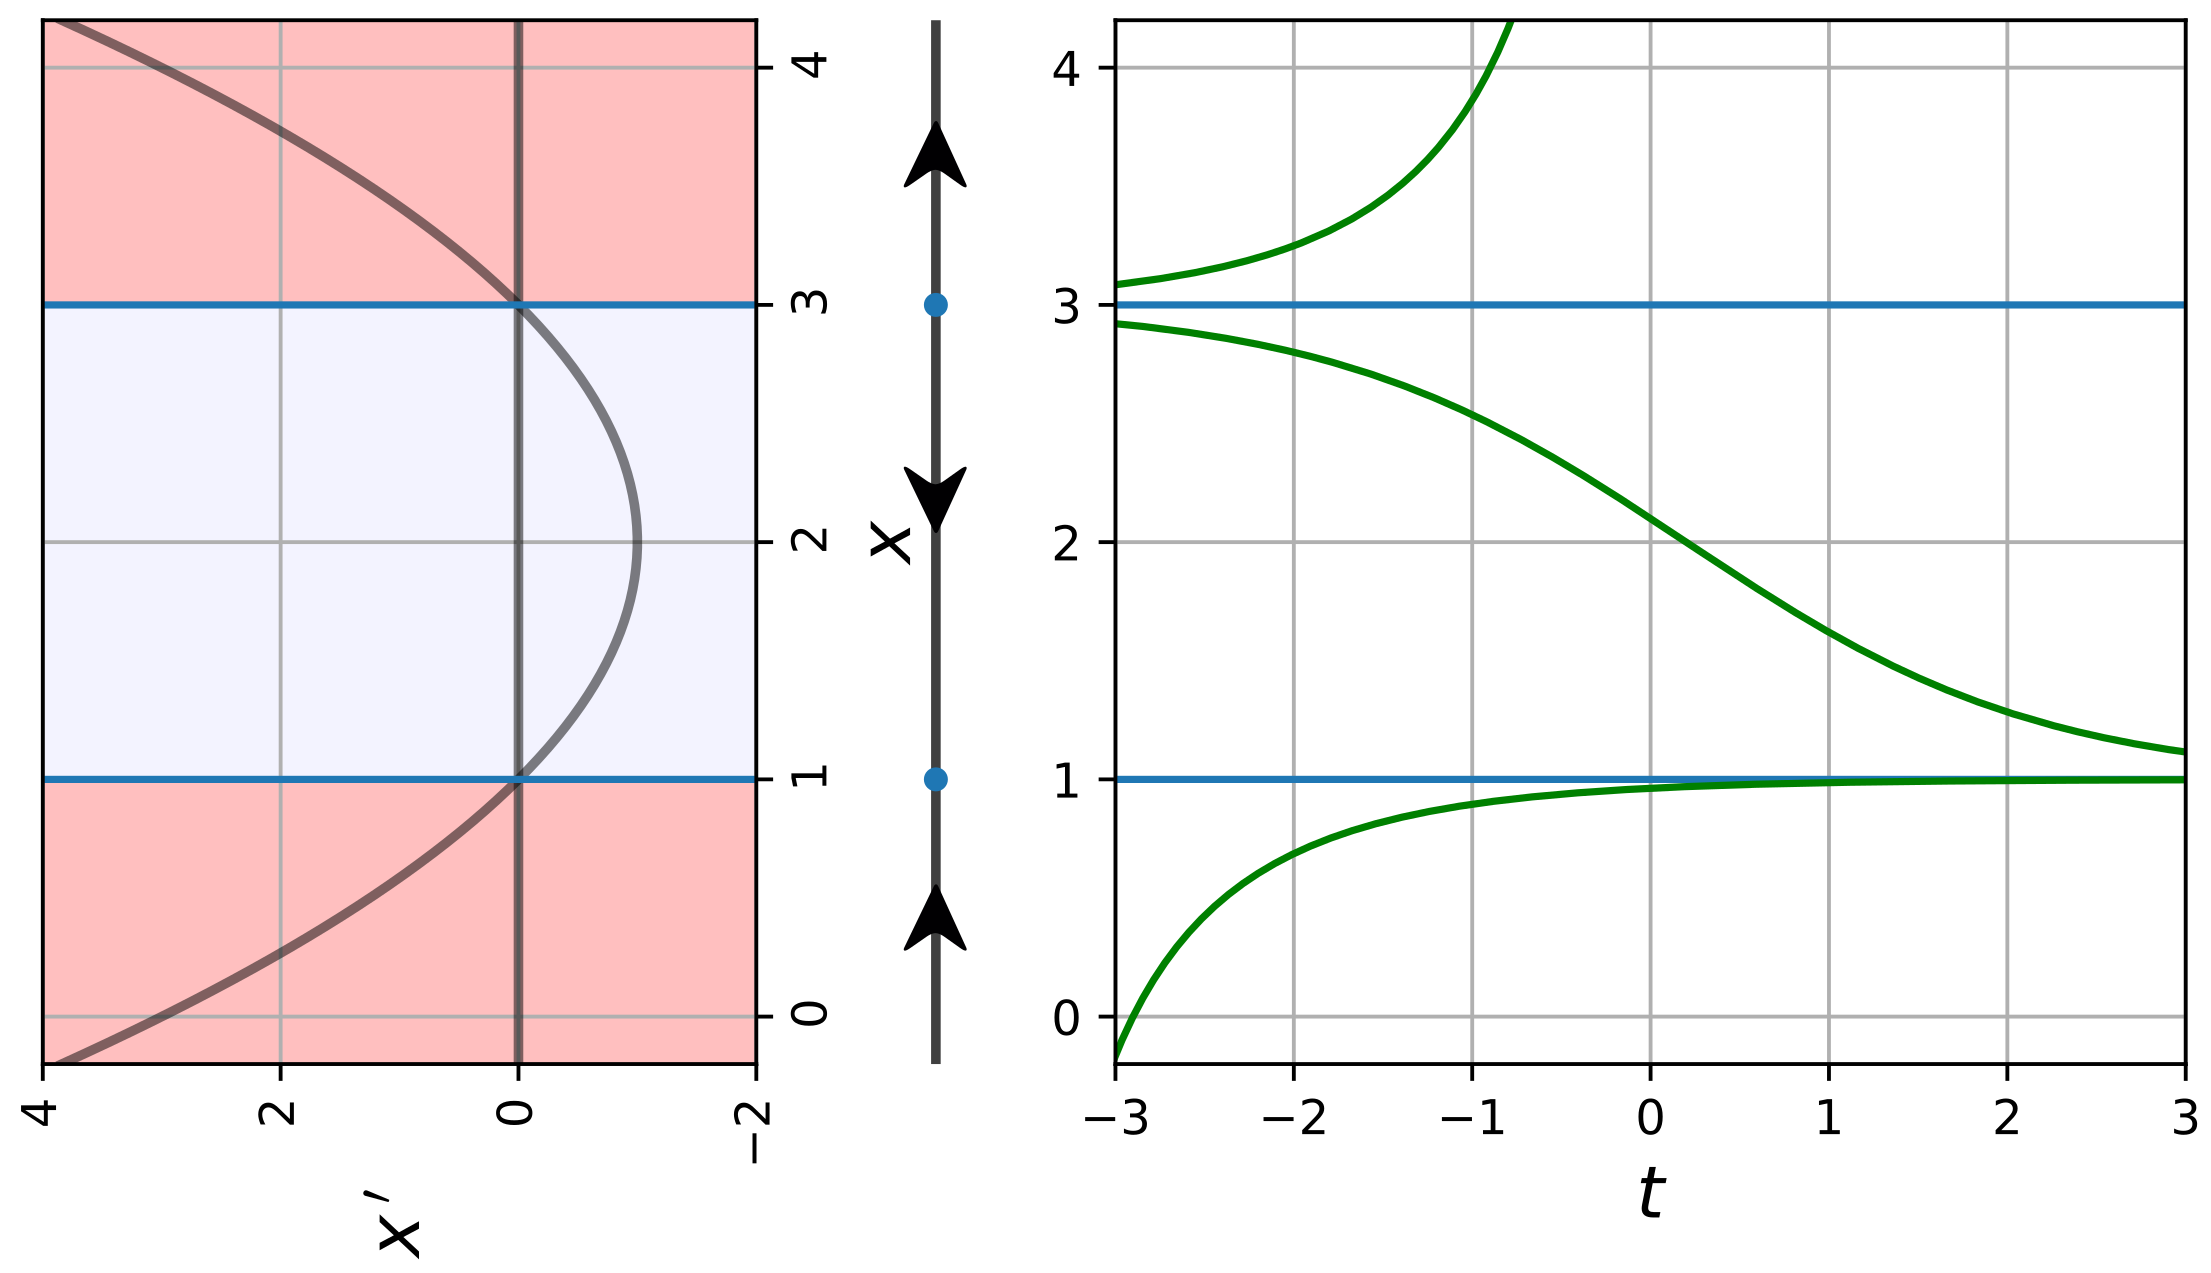
\includegraphics[width=6.0in, height=3.0in]{additional_figures/first_order_extra_figure_longer_time_update_202001.png}
\caption{}
\label{logisticredrawnjr}

\end{figure}

\item Sketch $x' = f(x)$ in the $xx'$-plane. Note that each value $x=c$ such that $f(c)=0$ corresponds to a constant solution 
$x(t)\equiv c$ for all $x$.
The values $x=c$ are also called  critical points or equilibria of the DE.

\item Mark the critical points $x = c$ as dots on the $x$-axis of the phase line.
These divide the phase line into subintervals.

\item Draw an arrow on each subinterval,
pointing up if $f>0$ on the subinterval and down if $f<0$.
%\item 
%For each CP, inspect the neighboring arrows on the phase line 
%and classify the CP as stable or unstable.
{\color{teal}BH skip classifying as stable/unstable}
\item
Sketch the constant solutions $x(t) \equiv c$ in the $tx$-plane.
These lines divide the $tx$-plane into subregions corresponding to
the subintervals of the phase line.

\item Select one IC $(t_0,x_0)$ for each different subregion 
 and sketch the corresponding solution.
Base the sketch on whether $x(t)$ is increasing or decreasing
as shown by the arrows on the phase line.
Each solution curve must lie entirely in one of the subregions.
It can be shown by using the Picard existence/uniqueness theorem for first order ODEs (Theorem \ref{slope:picardthm}) that different solution curves cannot intersect 
($y$ and $x$ of the Theorem correspond to $x$ and $t$ here, respectively).
It follows that each non-constant solution $x(t)$ cannot cross or even touch any of the lines $x=c$ because these lines represent constant solutions $x(t)\equiv c$.

\end{enumerate}
In the example shown in \figurevref{logisticredrawnjr}, each of the three non-constant solution curves  represents
a class of solutions having the same qualitative behavior:

\begin{enumerate}[1)]
    \item Any IC $(t_0,x_0)$ with $x_0 < 1$ 
    leads to a solution which is strictly increasing and asymptotic as $t\to\infty$ to $x\equiv 1$. 
    For $t<t_0$, the solution takes on arbitrarily large negative values.
    \item Any IC $(t_0,x_0)$ with $1 < x_0 < 3$ leads to a solution which is
    strictly decreasing for all $t$ and asymptotic as $t\to\infty$ to $x\equiv 1$. As $t\to-\infty$ the solution is asymptotic to $x\equiv 3$.
    \item Any IC $(t_0,x_0)$ with $x_0>3$ 
    leads to a solution which is
    strictly increasing. For  $t>t_0$, the solution takes on arbitrarily large positive values. As $t\to -\infty$,
    the solution is asymptotic to $x\equiv 3$.
    {\color{teal}BH solutions cease to exist at finite time, so as $t\to\infty$
    isn't correct}
\end{enumerate}
{\color{teal}BH strictly increasing is stronger than monotonic increasing-
the "monotonic" is unnecessary }
{\color{teal}BH removed erroneous "fix" of replacing (1,2) with (1,2]}

\end{example}

%extra exercises {Autonomous equations}

\begin{exercise}
%http://math.buffalo.edu/306/2019_06_19/001
%begin-exercise-prequel
\textit{Follow the steps in \exampleref{Autoeq:sketching auto} to sketch the qualitative-different solution curves for the following autonomous DEs. Be sure to show all key features of the three graphs, zeros of $f(x)$, arrows of increase / decrease, ..., as in \figurevref{logisticredrawnjr}.}
%end-exercise-prequel
$x' = x^2-6x+5$.
\end{exercise}

\begin{exercise}
%http://math.buffalo.edu/306/2019_06_19/002
$x' = -x^2+x+2$.
\end{exercise}

\begin{exercise}
%http://math.buffalo.edu/306/2019_06_19/003
$x' = x+3$.
\end{exercise}

\begin{exercise}
%http://math.buffalo.edu/306/2019_06_19/004
$x' = (x+2)^2$.
\end{exercise}

\begin{exercise}
%http://math.buffalo.edu/306/2019_06_19/005
$x' = -x^2+6x-9$.
\end{exercise}

\begin{exercise}
%http://math.buffalo.edu/306/2019_06_19/006
$x' = -2x+2$.
\end{exercise}

\begin{exercise}
%http://math.buffalo.edu/306/2019_06_19/007
$x' = x^2-4x+4$.
\end{exercise}

\begin{exercise}
%http://math.buffalo.edu/306/2019_06_19/008
$x' = -x^2+5x-4$.
\end{exercise}

\begin{exercise}
%http://math.buffalo.edu/306/2019_06_19/009
$x' = x^2-4$.
\end{exercise}

\begin{exercise}
%http://math.buffalo.edu/306/2019_06_19/010
$x' = -x^2+x+6$.
\end{exercise}

\begin{exercise}
%http://math.buffalo.edu/306/2019_06_19/011
$x' = (3-x)^3$.
\end{exercise}

\printanswers
\end{document}


